\chapter{VarBench: variational benchmarks for quantum many-body systems}
\label{ch:varbench}

In the previous chapters,

\rrc{push the figure on the second page!}

\begin{figure}[htb]
\centering
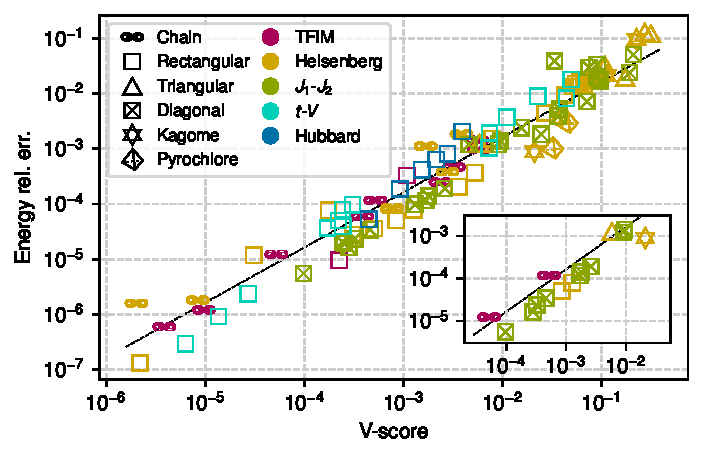
\includegraphics[width=0.8\linewidth]{ch10/v_score_rel_err.pdf}
\caption[Comparison of V-score and energy relative error]{
Comparison of V-score and energy relative error for systems whose exact solutions from ED or QMC are available.
The black dashed line is the least-squares fit.
The inset focuses on PQC results simulated on classical hardware without noise.
This figure is reproduced from Fig.~2 in Ref.~\cite{wu2023variational}.
}
\label{fig:v-score-rel-err}
\end{figure}

\begin{figure}[htb]
\centering
\hspace*{-0.05\linewidth}
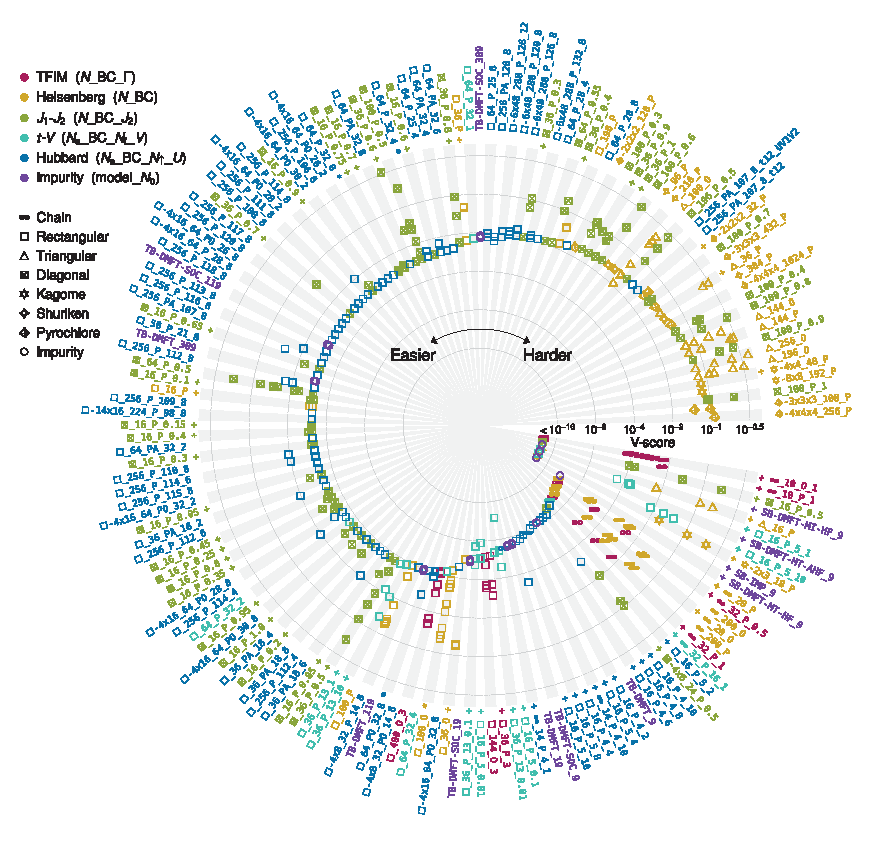
\includegraphics[width=1.05\linewidth]{ch10/v_score_polar_doubly_log.pdf}
\caption[Overview of VarBench results]{
Overview of the complete benchmark results.
Each slice in the radial direction contains different variational methods for a given Hamiltonian. The bold marker indicates the method with the lowest variational energy (rather than the lowest V-score), which defines the V-score for the Hamiltonian and determines its clockwise ranking.
The radial axis uses the doubly log scale to show the results across a wide range of V-score magnitude.
The results with V-scores less than $10^{-16}$ are indistinguishable from the exact solutions due to limited numerical precision.
The label outside each slice is the name of the Hamiltonian in the dataset, which describes the lattice geometry, the lattice size $N_\text{s}$, the boundary conditions (BC), and the Hamiltonian parameters such as the interaction strength ($\Gamma$, $J_2$, $V$, $U$) and the number of particles ($N_\mathrm{f}$, $N_{\uparrow}$, $N_\mathrm{b}$).
The BC can be O (open), P (periodic), A (anti-periodic) on each dimension.
The `\texttt{+}' marker near the label indicates that an ED solution is available for that Hamiltonian, and the `\texttt{\textasteriskcentered}' marker indicates a numerically exact QMC solution.
This figure is reproduced from Fig.~3 in Ref.~\cite{wu2023variational}.
}
\label{fig:v-score}
\end{figure}

\begin{figure}[htb]
\centering
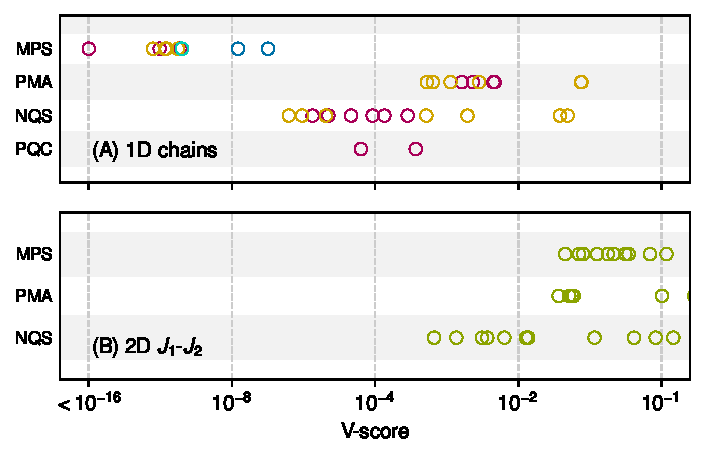
\includegraphics[width=0.8\linewidth]{ch10/v_score_method_doubly_log.pdf}
\caption[V-scores of different methods]{
V-scores classified by variational methods, including matrix product state (MPS), physically motivated ansatz (PMA), neural quantum state (NQS), and parameterized quantum circuit (PQC), on (a) 1D chains and (b) 2D $J_1$-$J_2$ models.
The $x$-axis uses the doubly log scale to show the results across a wide range of V-score magnitude.
}
\label{fig:v-score-method}
\end{figure}

\begin{figure}[htb]
\centering
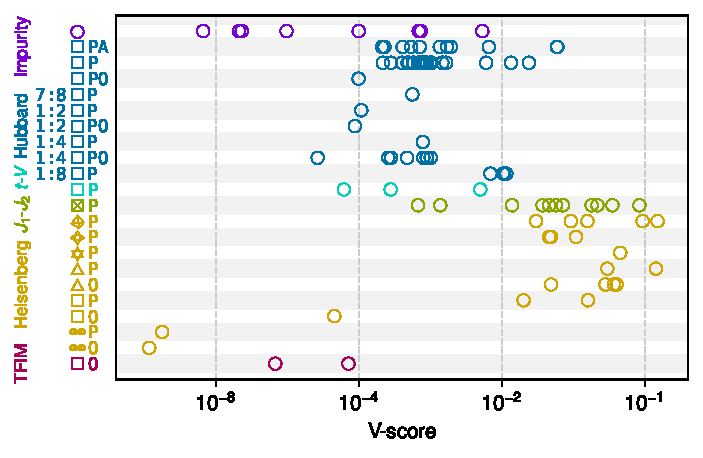
\includegraphics[width=0.8\linewidth]{ch10/v_score_ham_no_ed_doubly_log.pdf}
\caption[V-scores of different Hamiltonians]{
V-scores classified by Hamiltonian types and lattice geometries.
A Hamiltonian's V-score is defined as the V-score of the available variational method with the lowest energy on this Hamiltonian.
Only the Hamiltonians without ED results are shown.
The $x$-axis uses the doubly log scale to show the results across a wide range of V-score magnitude.
The ratios to the left of the lattice icons are aspect ratios of rectangular lattices. The letters to the right are boundary conditions, which can be O (open), P (periodic), A (anti-periodic) on each dimension.
This figure is reproduced from Fig.~4 in Ref.~\cite{wu2023variational}.
}
\label{fig:v-score-ham}
\end{figure}
